%% Requires compilation with XeLaTeX or LuaLaTeX
\documentclass[10pt,xcolor={table,dvipsnames},t]{beamer}
\usetheme{UCBerkeley}
\usepackage{tikz}
\usepackage{graphicx}
\usepackage{amsmath,amsthm,amssymb}
\usepackage{float}
\usepackage{comment}
\usepackage{tikz-cd}
\usepackage{setspace}
\usepackage{makecell}
\usepackage{physics}

\title[Your Short Title]{From Quasars to Quarks: Day 1.1}
\subtitle{Math Review}
\author{Charlie Cummings \& Shaunak Modak}
\institute{While you're waiting, fill this out: tinyurl.com/FQ2Q-math}
\date{August 31, 2020}

\begin{document}

\begin{frame}
    \titlepage
\end{frame}

\section{Introduction}

% play the video for powers of ten

\begin{frame}{Course Logistics}
    Welcome to FQ2Q!
    \vspace{-10pt}
    \begin{columns}
        \column{0.5\textwidth}
        \begin{itemize}
            \item $2$ unit PNP DeCal
            \item Course website: bcourses.berkeley.edu
            \item Grading:
                \begin{itemize}
                    \item HW: 5 pts, 2-3 problems weekly
                    \item Attendance: 1.5 pts per lecture
                    \item Final Project: 25 pts
                    \item 1 free pt :)
                    \item Need to collect 90/130 pts to pass
                \end{itemize}
            \item This is a fast paced course
            \item Come to office hours! (after class)
            \item Focus on the big picture!
            % BY THE END OF THIS COURSE, ...
        \end{itemize}
        \column{0.5\textwidth}
        \vspace{-50pt}
        \begin{figure}
            \centering
            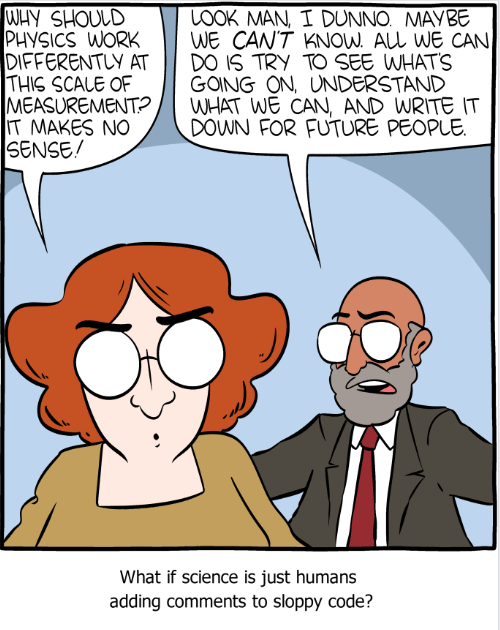
\includegraphics[scale=0.5]{smbc.png} \\
            \tiny{Source: https://www.smbc-comics.com/comic/how}
        \end{figure}
    \end{columns}
\end{frame}

\begin{frame}{Gather!}
    \begin{itemize}
        \pause \item Check it out at https://tinyurl.com/FQ2Q-class
    \end{itemize}
\end{frame}

\begin{frame}{Classroom Guidelines}
    \begin{itemize}
        \item Everyone has a right to be here and to learn!
        \item Be kind and respectful to your fellow students
        \begin{itemize}
            \item Intent vs. Impact
        \end{itemize}
        \item Let us know if you need any special accommodations
    \end{itemize}
\end{frame}

% Uncomment these lines for an automatically generated outline.
\begin{frame}{Outline}
    \tableofcontents
\end{frame}

\begin{frame}{Meet your Instructors!}
\begin{figure}
    \centering
    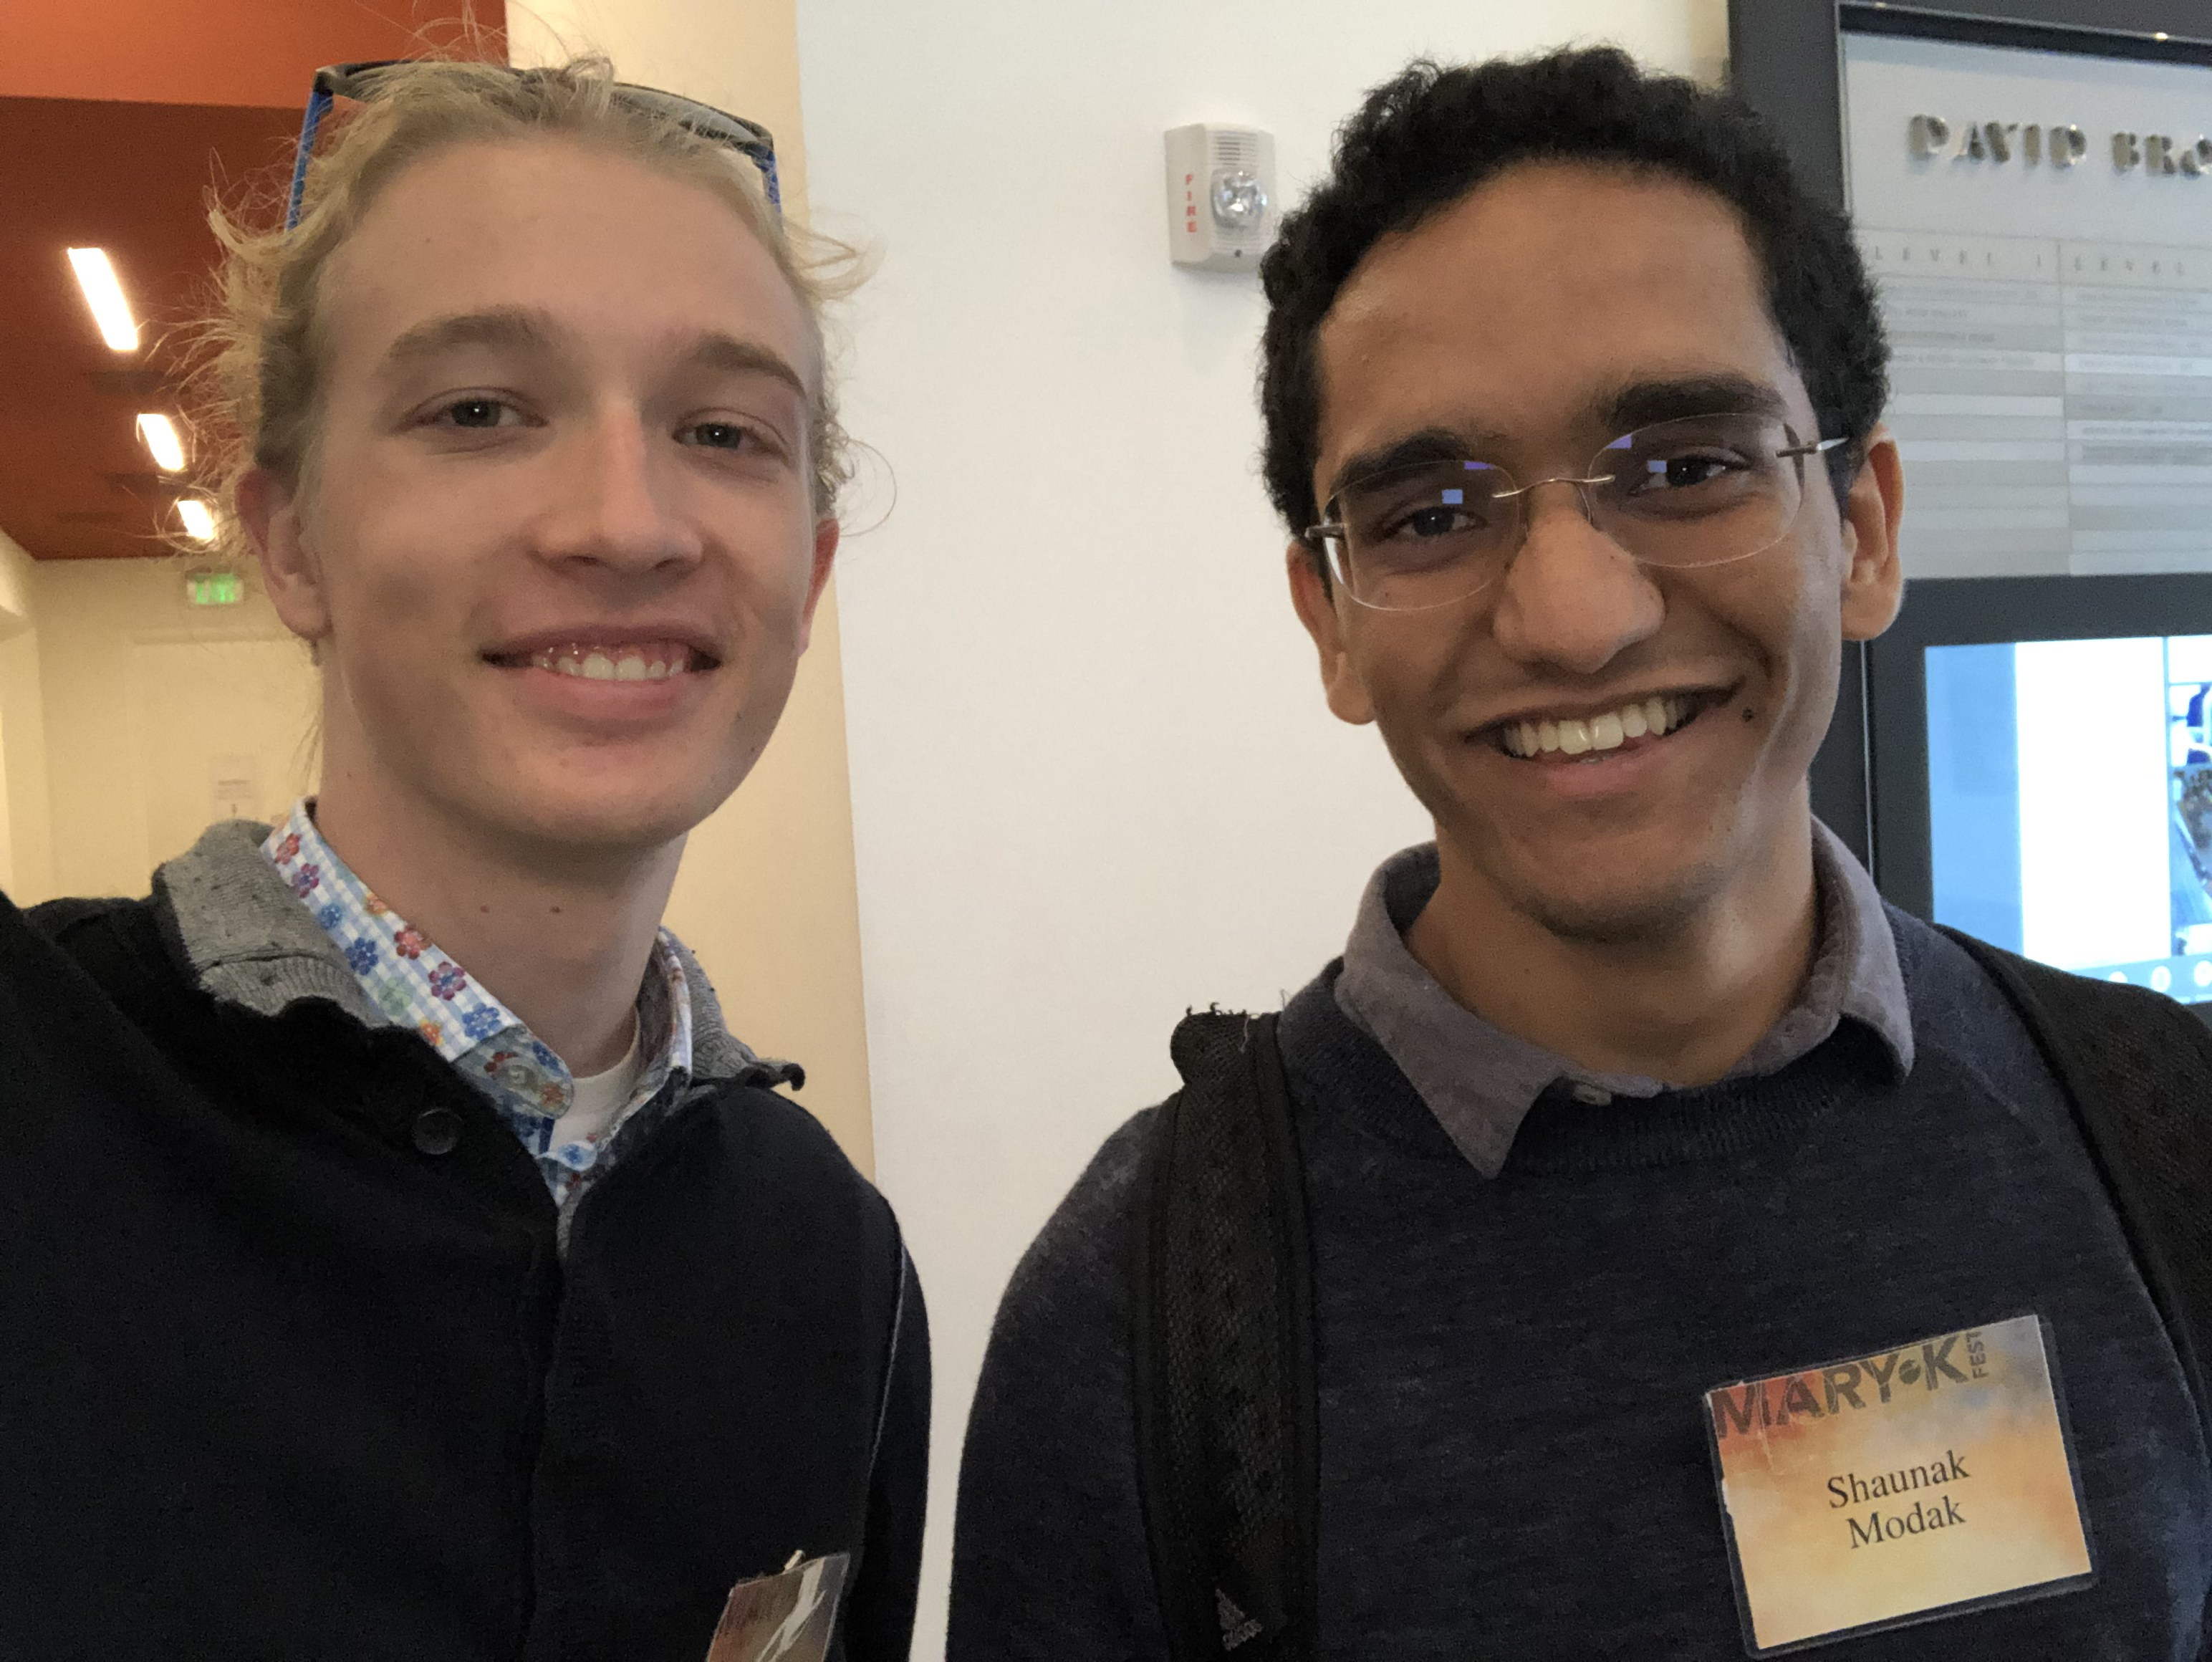
\includegraphics[scale=0.051]{IMG_0737_up.jpeg} \\
    \small{Friendship :)}
\end{figure}
    \begin{columns}[c]
        \column{.5\textwidth}
            \vspace{-5pt}
            \begin{itemize}
                \item Charlie Cummings (he/him)
                \item AMO, Particle, Nuclear, Cosmology 
                \item Scales [26,24] and [-8,-15]
            \end{itemize}
        \column{.5\textwidth}
            \vspace{-5pt}
            \begin{itemize}
                \item Shaunak Modak (he/him)
                \item Cosmology, Galaxies, Supernovae
                \item Scales [26, 8]
            \end{itemize}
    \end{columns}
\end{frame}

\section{Understanding Scales}

\begin{frame}{Answer to Attendance Question}
    \begin{itemize}
      \item Physics makes sense over (roughly) \textbf{60} orders of magnitude of length
    \end{itemize}

\end{frame}

\begin{frame}{Answer to Attendance Question}
    \begin{itemize}
      \item Physics makes sense over (roughly) \textbf{60} orders of magnitude of length
    \end{itemize}

    \begin{figure}
        \centering
        \def\omu{-35}
        \def\oml{-35}
        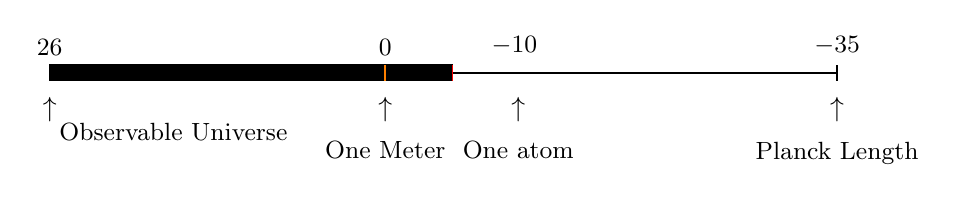
\begin{tikzpicture}
        
        %labels
        \node[anchor=south] at (-5,0.1) {\small $26$};
        %\node[anchor=south] at (-0.1639*\omu-0.7377,0.1) {\small $\omu$};
        %\node[anchor=north] at (-0.1639*\oml-0.7377,-0.1) {\small $\oml$};
        \node[anchor=south] at (-0.7377,0.1) {\small $0$};
        \node[anchor=south] at (0.1639*10-0.7377,0.1) {\small $-10$};
        \node[anchor=south] at (5,0.1) {\small $-35$};
        
        \node[anchor=south] at (-5,-0.75) {$\uparrow$};
        \node[anchor=west] at (-5,-0.75) {\small Observable Universe};
        
        \node[anchor=south] at (-.7377,-0.75) {$\uparrow$};
        \node[anchor=north] at (-.7377,-0.75) {\small One Meter};
        
        \node[anchor=south] at (0.9506,-0.75) {$\uparrow$};
        \node[anchor=north] at (.9506,-0.75) {\small One atom};
        
        \node[anchor=south] at (5,-0.75) {$\uparrow$};
        \node[anchor=north] at (5,-0.75) {\small Planck Length};
        
        %blue fill bar
        \filldraw (-5,0.1) -- (-0.1639*\omu-0.7377,0.1) -- (-0.1639*\omu-0.7377,-0.1) -- (-5,-0.1) -- cycle;
        %red fill bar
        \filldraw[red] (-0.1639*\omu-0.7377,-0.1) --  (-0.1639*\omu-0.7377,0.1) -- (-0.1639*\oml-0.7377,0.1)--(-0.1639*\oml-0.7377,-0.1) -- cycle;
        %blue thin bar
        \draw[thick] (-0.1639*\oml-0.731,0) -- (5,0);
        %vertical blue thin bar
        \draw[thick] (5,.1) -- (5,-.1);
        %1m mark
        \draw[thick, orange] (-0.7377,.1) -- (-0.7377,-.1);
    
        \end{tikzpicture}
        \caption{$\log_{10}\left(\frac{L}{1 m}\right)$}
        \label{fig:progress}
    \end{figure}


    %\item The Birth/Death of the Entire Universe, \textbf{Quasars}, Black Holes, Exoplanets, Neurons, Matter, Antimatter, \textbf{Quarks}, String Theory

\end{frame}

\section{Units and Dimensional Analysis}

\begin{frame}{Relative vs Absolute Changes}

\begin{itemize}
  \item $a+b = a\left( 1 + \frac{b}{a}\right)$
  \item $a$ carries the units (and therefore the scale) of the problem and $\frac{b}{a}$ tells how much things change
  \item $f(x)g(x) = e^{\ln{fg}} = e^{\ln{f}\left( 1 + \frac{\ln{g}}{\ln{f}}\right)}$
  \item $\frac{d}{dt}(fg) = \dot{f}g + f\dot{g} = \left( \frac{\dot{f}}{f} + \frac{\dot{g}}{g} \right) fg$
\end{itemize}

\end{frame}

\begin{frame}{Units and Dimensional Analysis}
    \begin{itemize}
        \item Why does $1kg*1\frac{m}{s}$ make sense but $1kg + 1\frac{m}{s}$ doesn't?
        %global scaling!
    \end{itemize}
\end{frame}

\begin{frame}{Dimensionless Quantities are What Matter}
    \begin{itemize}
        \item $\omega = \sqrt{\frac{g}{L + x}}$
        \item $T = \frac{mgR^2}{R^2 + 2b^2}$
        \item $ds^2 = \left(1 - \frac{2GM}{c^2 r}\right)c^2dt^2 - \frac{dr^2}{\left(1 - \frac{2GM}{c^2 r}\right)} - r^2 d\Omega^2$
    \end{itemize}
\end{frame}

\begin{frame}{Dimensionless Quantities are What Matter}
    \begin{itemize}
        \item $\omega = \frac{1}{\sqrt{1 + \frac{x}{L}}} \sqrt{\frac{g}{L}} = \frac{\omega_0}{\sqrt{1 + \frac{x}{L}}} \implies \frac{\omega}{\omega_0} = \frac{1}{\sqrt{1 + \frac{x}{L}}} $
        \item $\frac{T}{mg} = \frac{1}{1 + 2\left(\frac{b}{R}\right)^2}$
        \item $ds^2 = \left(1 - \frac{R_s}{ r}\right)c^2dt^2 - \frac{dr^2}{\left(1 - \frac{R_s}{ r}\right)} - r^2 d\Omega^2$
    \end{itemize}
\end{frame}

\begin{frame}{Approximations}
    \begin{itemize}
        \item Physicists love approximations, but why?
        \item Tractability of equations
        \item How can we simplify things?
    \end{itemize}
\end{frame}

\begin{frame}{Approximations}
    \begin{itemize}
        \item Physicists love approximations, but why?
        \item Tractability of equations
        \item How can we simplify things?
        \begin{itemize}
            \item Taylor Series
        \end{itemize}
    \end{itemize}
\end{frame}

\begin{frame}{Approximations}
    \begin{itemize}
        \item Physicists love approximations, but why?
        \item Tractability of equations
        \item How can we simplify things?
        \begin{itemize}
            \item Taylor Series
            \item Perturbations
        \end{itemize}
    \end{itemize}
\end{frame}

\begin{frame}{Approximations}
    \begin{itemize}
        \item Physicists love approximations, but why?
        \item Tractability of equations
        \item How can we simplify things?
        \begin{itemize}
            \item Taylor Series
            \item Perturbations
            \item Limits (``regimes'')
        \end{itemize}
    \end{itemize}
\end{frame}

\begin{frame}{Fundamental Constants}
    %list them
    \begin{itemize}
        \item Universal conversion factors
        \item Just like $\frac{5280 \textrm{ft}}{1 \textrm{mile}}$ is a universal conversion factor...
        \item Units based on these?
    \end{itemize}
\end{frame}

\begin{frame}{Planck Units}
    \begin{itemize}
        \item Use units where all fundamental constants are $1$
    \end{itemize}
    
    \begin{tabular}{|c|c|c|c|}
        \hline 
        Name & Dimension & Expression & Value in SI units  \\
        \hline
        \hline
        Planck Length & [L] & $l_P = \sqrt{\frac{\hbar G}{c^3}}$ & $\approx 1.6 \times 10^{-35}$m \\
        Planck Time & [T] & $t_P = \sqrt{\frac{\hbar G}{c^5}}$ & $\approx 5.4 \times 10^{-44}$s \\
        Planck Mass & [M] & $m_P = \sqrt{\frac{\hbar c}{G}}$ & $\approx 2.2 \times 10^{-8}$kg \\
        Planck Temperature & [$\Theta$] & $T_P = \sqrt{\frac{\hbar c^5}{k_B^2 G}}$ & $\approx 1.4 \times 10^{32}$K \\
        \hline
    \end{tabular}
\end{frame}

\begin{frame}{Units and Functional Form}
    \begin{itemize}
        \item $E = mc^2$
        \item $p = \frac{h}{\lambda}$
        \item $F_G = G \frac{m_1 m_2}{r^2}$
    \end{itemize}
\end{frame}

\begin{frame}{Units and Functional Form}
    \begin{itemize}
        \item $\frac{E}{E_p} = \frac{m}{m_p}$
        \item $\frac{p}{p_p} = \frac{l_p}{\lambda}$
        \item $\frac{F_G}{F_p} = \frac{l_p^2}{m_p^2}\frac{m_1 m_2}{r^2}$
    \end{itemize}
\end{frame}

\section{Math Review}

\begin{frame}{Math Review: Complex Numbers}
% quick review: stuff works like reals, but 2D; draw plane with a point as a + bi and re^i\theta, Euler's formula
% parametrizing unit circle with e^i\theta, what multiplication means as rotation
\end{frame}

\begin{frame}{Math Review: Vectors}
% vector addition, scaling, etc. and column vs row vectors / intro to multiplication rule of row times column, basis vectors & how to write things in terms of the basis, etc.
\end{frame}

\begin{frame}{Math Review: Multivariable Calculus}
% partial derivatives, multi chain rule
% div grad curl definitions
% what it means to integrate over a line/surface/volume
% idea behind stokes theorem stuff
\end{frame}

\begin{frame}{Math Review: Matrices}
% what is a matrix (origin w/ linear equations)
% how to compute matrix multiplication, rules for scalar mult and composition etc. (linear transformations, viewed as functions on vectors)
% how it's not commutative / the commutator notation
% hint at how they're like vectors themselves (HW)
% the identity matrix and the concept of inverses
% transposes/daggers, def of Hermitian/Unitary etc.
% determinant, trace
\end{frame}

\begin{frame}{Math Review: Eigenstuff}
% start with diagonal matrices: normal basis vectors are eigenvectors and diag entries are eigenvalues bc ...
% Write in a new basis: more complex
% eigen means special!
\end{frame}

\begin{frame}{Math Review: Einstein Notation}
% what a vector, matrix, matrix multiplication etc look like in this
% big emphasis on the repeated index is summed over, very explicit
\end{frame}

\section{Takeaways}

\begin{frame}{Takeaways}
    \begin{itemize}
        \item Different physics is important at different length scales
        \item Units are important, but physics is secretly built on dimensionless quantities
        \item Breaking a problem into relative and absolute quantities is a crucial skill
        \item Math is the language of physics!
    \end{itemize}
\end{frame}

\end{document}
